\documentclass{egpubl}
\usepackage{eg2013}

% --- for  Annual CONFERENCE
% \ConferenceSubmission   % uncomment for Conference submission
% \ConferencePaper        % uncomment for (final) Conference Paper
% \STAR                   % uncomment for STAR contribution
% \Tutorial               % uncomment for Tutorial contribution
% \ShortPresentation      % uncomment for (final) Short Conference Presentation
% \Areas                  % uncomment for Areas contribution
\MedicalPrize           % uncomment for Medical Prize contribution
% \Education              % uncomment for Education contribution
%
% --- for  CGF Journal
% \JournalSubmission    % uncomment for submission to Computer Graphics Forum
% \JournalPaper         % uncomment for final version of Journal Paper
%
% --- for  EG Workshop Proceedings
% \WsSubmission    % uncomment for submission to EG Workshop
% \WsPaper         % uncomment for final version of EG Workshop contribution
%
 \electronicVersion % can be used both for the printed and electronic version

% !! *please* don't change anything above
% !! unless you REALLY know what you are doing
% ------------------------------------------------------------------------

% for including postscript figures
% mind: package option 'draft' will replace PS figure by a filname within a frame
\ifpdf \usepackage[pdftex]{graphicx} \pdfcompresslevel=9
\else \usepackage[dvips]{graphicx} \fi

\PrintedOrElectronic

% prepare for electronic version of your document
\usepackage{t1enc,dfadobe}

\usepackage{egweblnk}
\usepackage{cite}
\usepackage{flushend}
\usepackage{subfigure}
\usepackage{graphicx}
\usepackage{color}

\newcommand{\red}[1]{{\color{red}{#1}}}
\newcommand{\fix}[1]{\red{\emph{#1}}}
\newcommand{\Fix}[1]{\begin{itemize} \renewcommand\labelitemi{\red{--}} \item \red{#1} \end{itemize}}

% For backwards compatibility to old LaTeX type font selection.
% Uncomment if your document adheres to LaTeX2e recommendations.
% \let\rm=\rmfamily    \let\sf=\sffamily    \let\tt=\ttfamily
% \let\it=\itshape     \let\sl=\slshape     \let\sc=\scshape
% \let\bf=\bfseries

\title{Guiding Deep Brain Stimulation Interventions by Fusing Multimodal Uncertainty Regions}

\author[Bock et al.]{
Alexander Bock$^1$,
Norbert Lang$^2$,
Ralph Lehrke$^2$,
and Timo Ropinski$^1$\\
$^1$Scientific Visualization Group, Link\"oping University, Sweden\\
$^2$Stereotactic Neurosurgery, St. Barbara Klinik, Hamm-Heessen, Germany
}

\begin{document}
\maketitle
\begin{abstract}
Deep Brain Stimulation (DBS) is a surgical intervention that is known to reduce or eliminate the symptoms of common movement disorders, such as Parkinson's disease, dystonia, or tremor by implanting stimulating electrodes into specific regions. We present a system that combines the currently unconnected information channels into a unified system. This enables the surgical team immediate access to preoperative imaging data, Microelectrode Recordings, and patient feedback, which reduces the time in the operating room and increases the precision of the placed electrode. Furthermore, it will allow the surgeon to perform post-operation analyses to improve the currently employed operational heuristics.
\begin{classification}
\CCScat{Computer Graphics}{I.3.3}{foo}{bar}
\end{classification}
\end{abstract}

\section{Introduction}\label{sec:introduction}
Due to advances in medicine, society is now facing the problems of an aging population suffering from an increasing occurrence of age-related diseases like \emph{movement disorders} such as Parkinson's Disease (PD), dystonia, or tremors that greatly affect the patients' quality of life. As both symptoms affecting motor skills, and the psychological consequences of these diseases have a great impact on everyday life, successful treatment strategies are of increasing importance.

Deep Brain Stimulation (DBS) is a procedure for reducing the symptoms of these diseases~\cite{Benabid2009} and capable of improving the overall quality of life in the cases where medication is not a viable option. To conduct a DBS, electrodes are implanted into specific regions of the brain and then emit electrical signals to stimulate these regions. In the case of PD the most effective target areas for electrode placement are the subthalamic nuclei (STN) with sizes of a few millimeters. As misplaced stimulation electrodes can have severe side effects, including speech difficulties, increased tremor, or long term memory problems, accurate electrode placement is crucial. Nowadays the access path to the target region is planned using a combination of magnetic resonance imaging (MRI) and an atlas-based heuristic to locate the STN. To further verify the electrode placement, the patient performs simple tasks during the operation that are monitored by the surgical staff. Depending on the location of the electrode, a different region of the brain is stimulated, resulting in measurable responses from the patient. These responses can be cognitive, e.\,g.,~memory impairment, or motor-related, e.\,g.,~increased tremor or speech impairment. To further reduce the uncertainty of the electrode placement intra-operative x-ray scans can be performed to confirm the electrode placement.

In recent years Microelectrode Recording (MER) has emerged as an additional technique allowing the surgeon to better locate the target region for DBS intra-operatively~\cite{Lenz1988}. MER measures the electrical field of the brain during the surgery by inserting electrodes into the access path. The measured information is presented to the surgical staff by showing the amplitude in the time domain for each electrode, from which the expert can differentiate functional regions of the brain. In order to allow for an intuitive and accurate placement of the electrodes, it is important that the surgeon has access to all these modalities in a unified manner.

Our interactive visualization system supports the surgical team in two ways. One, by integrating the different modalities into a unified system, we enable faster and more reliable access to necessary information. This increases the accuracy and precision of the placement and reduces the time spent during the operation. Since the patient is awake during the procedure and under a lot of physical stress, this aspect is as desirable to achieve. Two, storing all the data acquired during the operation and being able to review past operations will enable new research opportunities towards improving the patient-neutral heuristic to locate the STN.

The rest of the paper is structured as follows: the next section will give a brief overview of the DBS procedure and then present the important views and techniques that were developed to create the system. Section~\ref{sec:benefits} will elaborate on the medical benefits of these techniques and relate them to the current systems. This will include an evaluation we have performed on 5 neurosurgeons. Section~\ref{sec:conclusion} will conclude the paper.

%To address this, we provide two views enhancing the final placement of the electrode by employing two separate fusion techniques. In the first view, we combine the structural and functional information about the target region gathered from different sources, such as pre-operative scans, x-ray scans, MER, patient checks, and present them to the surgeon in order to guide him to the optimal placement location. The view fuses this data with the structural information surrounding the intended target region in a multimodal visualization. This enables a mental registration of the measured data with the imaging modalities and, thereby, provides context that the surgeon can draw upon during the placement decision. In the second view we fuse the information about the occurring uncertainty and provide an information visualization approach to present the data in a quantitative way. The original data and derived information is presented as profile plots allowing the surgeon to see the optimal placement position at one glance and, thus, enable a more effective placement of the electrode.

%\section{Related Work}\label{sec:relatedwork}
%A visualization system for the pre-operative planning was provided by Beyer et al., who proposed a multi-volume renderer employing cut-away views to allow for visual access to the brain structures of interest~\cite{Beyer2007}. Furthermore, they included a skull peeling algorithm, which we have also incorporated into our system. Serra et al. created a neurosurgery planning tool for tumor resections, that uses a virtual workbench to increase user immersion and which provides additional 3D interaction tools~\cite{Serra1998}. Watanabe~et~al. developed a computer assisted surgery tool to treat cortical lesions, and used a curvilinear reformatting to allow direct access to the data~\cite{Watanabe}.  More recently, Rieder et al. proposed a planning tool for neurosurgical tumor treatment, that uses a cylindrical cut for a better view of the target region~\cite{Rieder2008}. Additionally, they introduce a distance ring to denote the relative depth of a specific region of interest. Furthermore, the same authors introduce visualization techniques to enhance the perception of structures when using multimodal rendering setups~\cite{Rieder2008a}.

%In the area of MER data integration Miocinovic et al. provide a system for a guided DBS electrode implantation in non-human~\cite{Miocinovic2007} as well as in human primates~\cite{Cicerone2}. They utilitize metaphors for visualizing region information but base the information on a 3D atlas only instead of using the MER signal. They also do not employ patient checks for feedback. In contrast, we provide a unified guidance system based on multi-modal measurements. Furthermore, their main focus is MER-based region detection for generating an atlas of the brain. D'Haese et al. presented a system for use in human surgery but focus on the comparison between MER selected targets and atlas-based target selection~\cite{Haese2005}. They also do not incorporate the patient test information into their system, which is required for a sufficient level of accuracy and confidence. Sperka et al. also presented a system to improve the planning phase for stereotaxic surgery~\cite{Sperka2011}. Lastly, the use of fMRI data together with other modalities was investigated in the context of stereotactic interventions on macaques~\cite{Ohayon2012}.

\section{System Overview}\label{sec:setup}
\begin{figure*}[t]
    \centering
    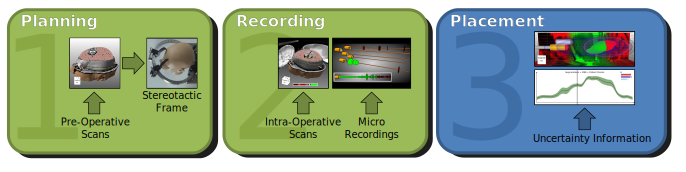
\includegraphics[width=0.8\linewidth]{figures/workflow}
    \caption{The workflow of the proposed DBS intervention system can be divided into three phases: planning, recording and placement. To support each of these phases, we employ dedicated views that are arranged in a multiple view setup as shows in Figure~\ref{fig:screenshot}. External components interacting with our visualization system are shown for each phase.}
    \label{fig:workflow}
\end{figure*}

%\fix{A DBS intervention can be divided into roughly three subsequent phases: \emph{planning}, in which the intended target region is selected, \emph{recording}, in which the MER signal is obtained, and \emph{placement}, in which the emitting electrode is inserted, the patient checks are performed, and the placement is evaluated (see also Figure~\ref{fig:workflow}). In the \emph{Planning Phase}, the desired target region is identified based on pre-operative scans, and a trajectory reaching that target region is planned which minimizes the distance to critical structures. There are a number of highly specialized tools available to perform this task, and since our focus is on other parts of the procedure, we implemented a basic planning tool, capable of importing the data from more sophisticated tools. In the \emph{Recording Phase}, the electrodes are advanced towards the target region, while each detects the signals from the surrounding tissue and transmits them to the controlling device. To obtain knowledge about the current region, the received signals are constantly analyzed and classified. In the \emph{Placement phase} the surgeon needs to consider all acquired information to determine the optimal position of the stimulating electrode. This decision is based on three different factors that are all affected by varying uncertainties:}

A DBS intervention can be divided into three subsequent phases: \emph{planning}, in which the intended target region is selected based on pre-operative scans, \emph{recording}, in which the MER signal is obtained, and \emph{placement}, in which the emitting electrode is inserted, the patient checks are performed, and the placement is evaluated (see also Figure~\ref{fig:workflow}).

%Figure~\ref{fig:screenshot} shows screenshots of the three different phases




\begin{figure}[t]
  \centering
%  \begin{minipage}[b]{0.45\columnwidth}
%  \subfigure{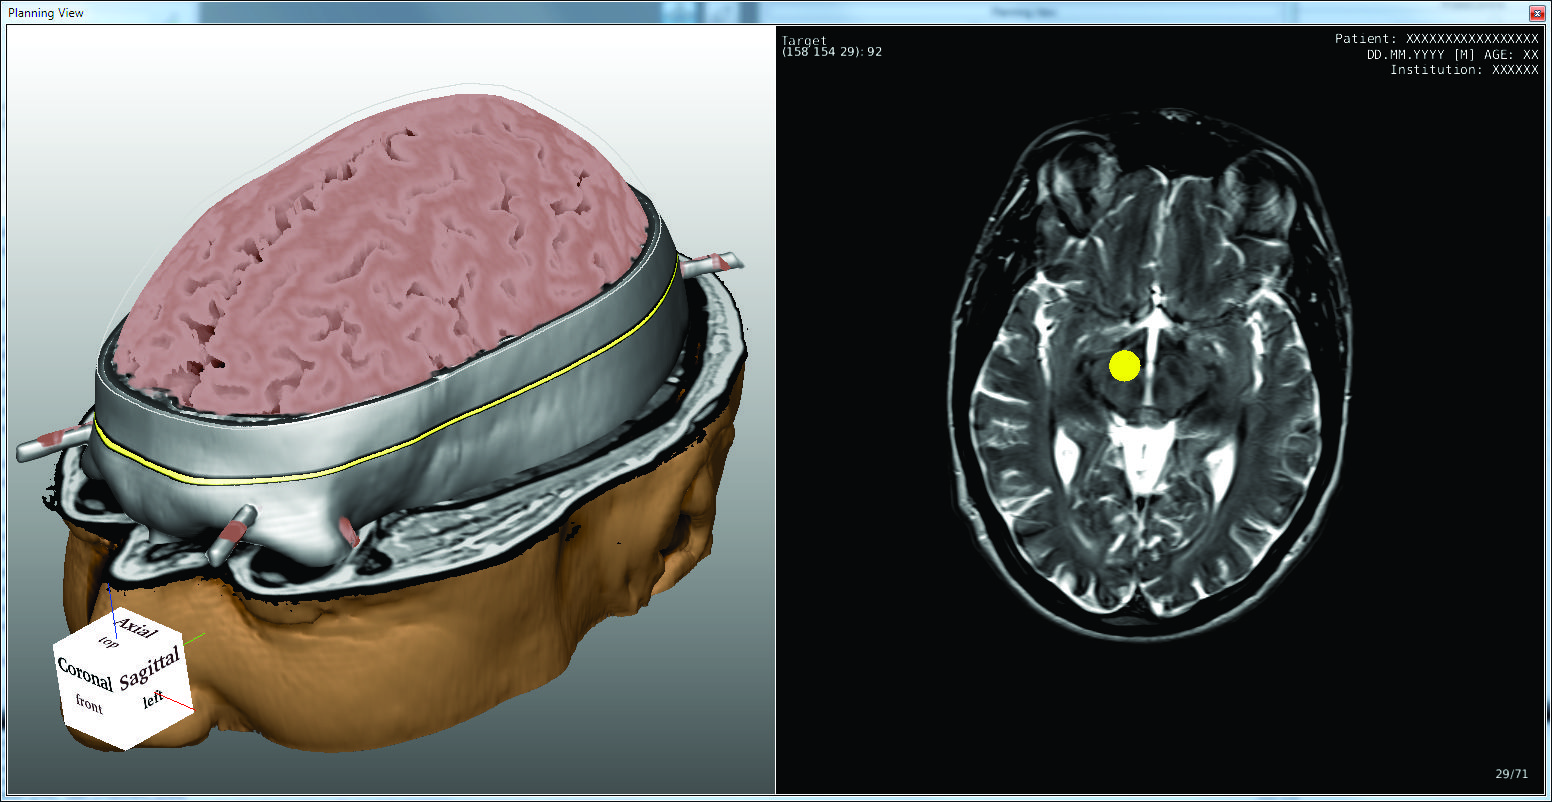
\includegraphics[width=\columnwidth]{figures/screenshot-planning.jpg}}\\
%  \vspace*{-0.02cm}
%  \subfigure{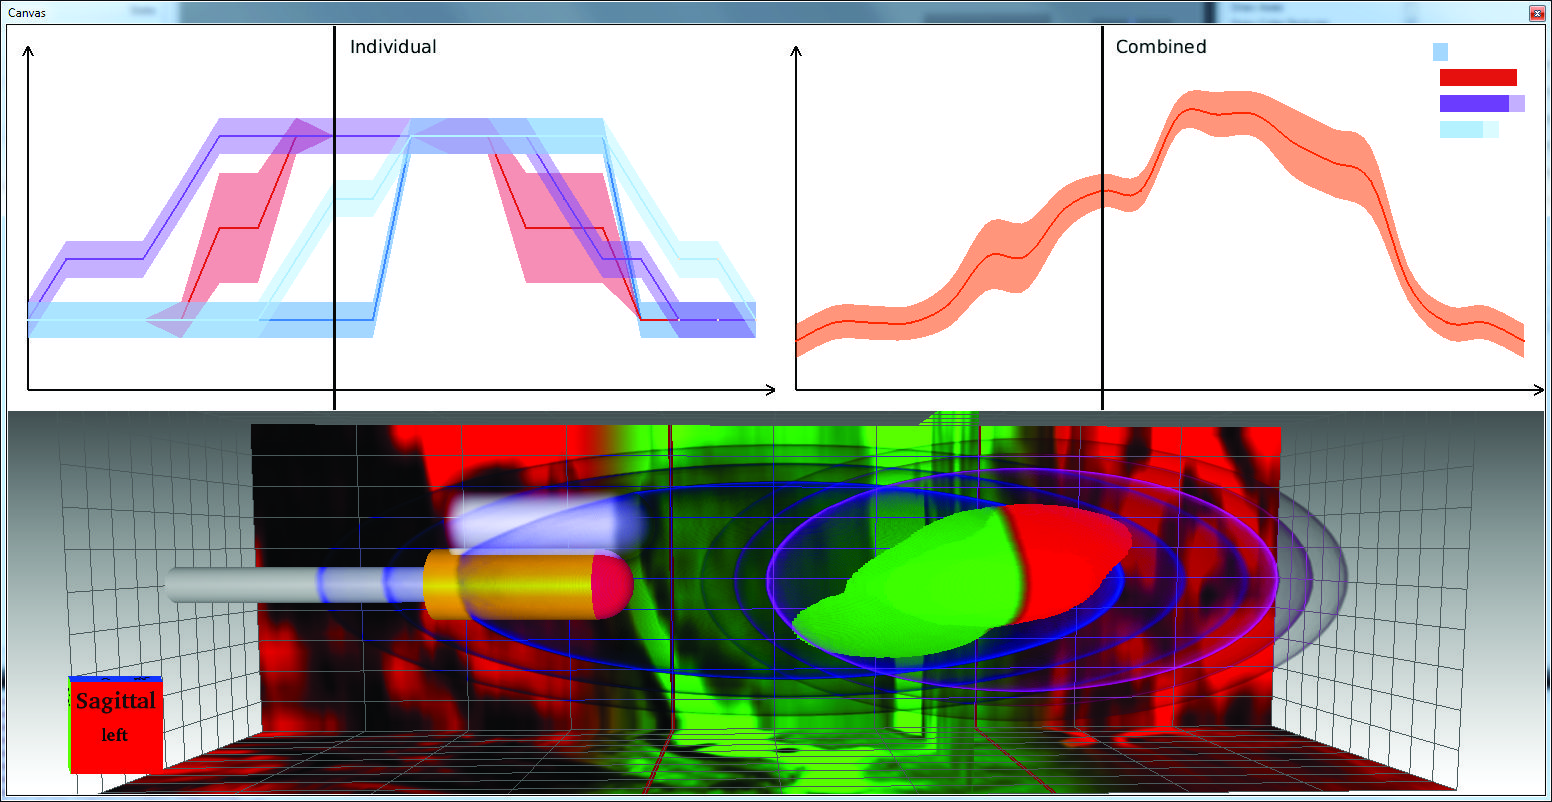
\includegraphics[width=\columnwidth]{figures/screenshot-target.jpg}}\\
%  \end{minipage}
  \subfigure{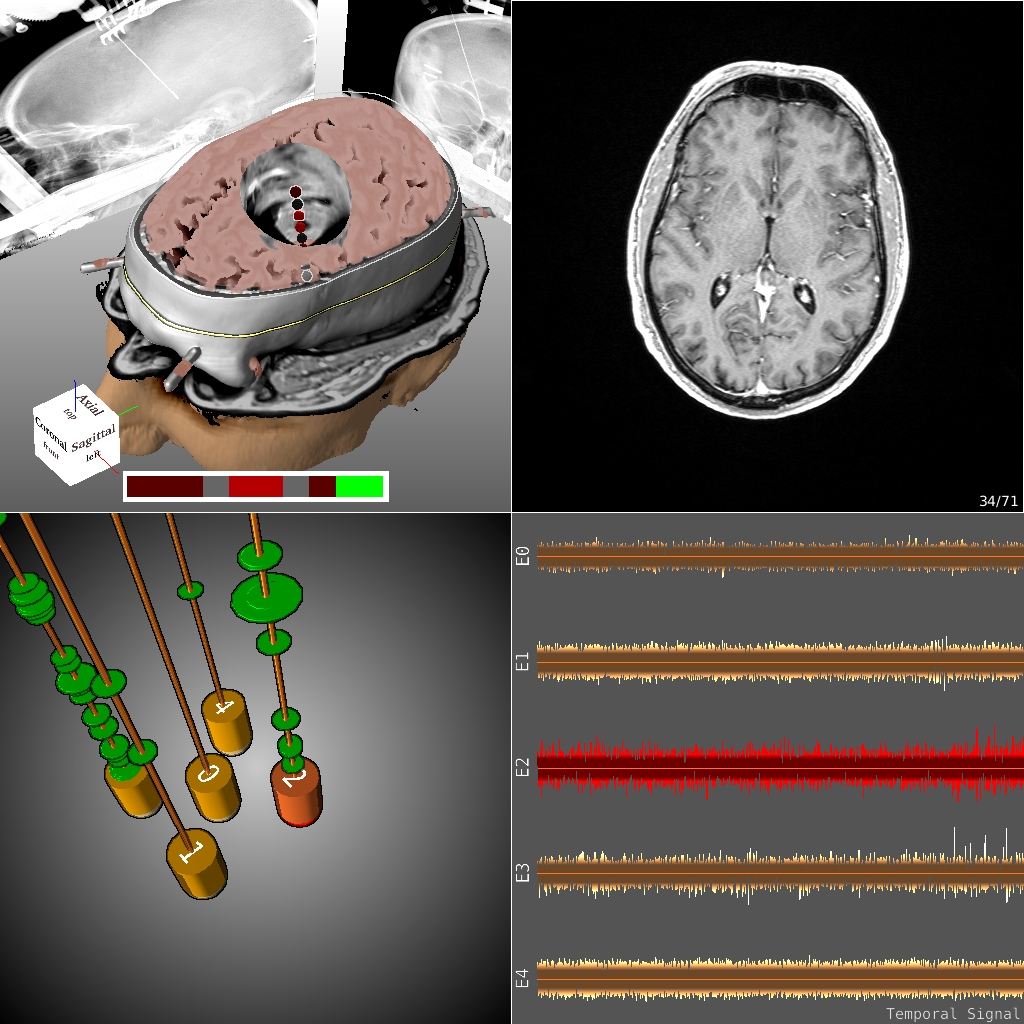
\includegraphics[width=\columnwidth]{figures/screenshot-recording.jpg}}
  \caption{Screenshots of our system during the recording phase.}
  \label{fig:screenshot}
\end{figure}

%The main goal of the designed system is to support the surgeon by reducing cognitive load by fusing the available modalities and thus facilitating mental registration~\cite{Tory1998}. The current situation in the operating theater is that the methods for inspecting the structural modalities, such as MRI, CT, and biplanar x-ray scans, are fairly advanced and widely used. However, the systems for recording and analyzing the MER signals and patient checks are decoupled from the other modalities. This forces the operating team to perform tasks serially, which prolongs the tiring procedure for the patient. By integrating the temporal data of the recording in the spatial context of the scans, the surgeon is relieved of the burden of mental registration and can perform the operation faster and with greater confidence.

%The second method through which we support the electrode placement is to present all collected data in a unified way, and show it in such a way that the optimal placement location is immediately visible and the surgeon is guided towards it. The collected data consists of information about the intended target region, the MER recording, patient checks, and their associated uncertainties.

%The traditional use of a planning system and an MER system side by side allows for the mental coregistration of MER signals, but this requires high levels of concentration fromt the surgeon. The situation is made worse because up to five parallel trajectories maybe recorded at the same time. Correlation of the MER signal of interest with the corresponding trajectory (for example anterior, posterior lateral central or medial) becomes a confusing task for the surgeon. The simple and intuitive display of a significant MER signal within the space of the planned trajectory is therefore a new feature with direct clinical benefit.   

%\subsection{DBS Intervention Procedure}\label{sec:overview:procedure}
%Before describing our system, we will first give a high-level overview of the DBS intervention procedure as it is specified in surgery guidelines~\cite{Hemm2010}. With respect to the steps in this procedure a DBS intervention can be divided into roughly three subsequent phases: \emph{planning}, in which the intended target region is selected, \emph{recording}, in which the MER signal is obtained, and \emph{placement}, in which the emitting electrode is inserted, the patient checks are performed, and the placement is evaluated (see also Figure~\ref{fig:workflow}). %As these three phases define the overall workflow of a DBS intervention, they are used as the blueprint for the workflow underlying the presented system (see Figure~\ref{fig:workflow}).

%As accuracy is of uttermost importance when performing DBS interventions, the patient is mounted into a stereotaxic frame that is rigidly fixed to the patient's skull. This frame has sockets that hold and precisely guide the equipment used during the intervention. Due to the known geometry of the stereotaxic frame, it serves as the basis for the coordinate transformation from imaging data to the patient. An important property of the frame is that it is visible in both CT and MRI scans, and can thereby serve as one of the landmarks used in the registration process. In the \emph{planning phase} the surgeon plans the access path based on the pre-operatively acquired T$_1$- and T$_2$- weighted MRI scans. In most cases, however, the target region is not directly visible on either of the MRI scans and the surgeon has to rely on experience and patient-neutral heuristics to locate the target area. This step introduces some uncertainty, of an unknown scale, into the position of the intended target region. %All these steps are performed within the planning phase of the DBS intervention. We will describe the visualization metaphors that we have developed to support this phase in Section~\ref{sec:overview:planning}.

%\begin{figure}[b]
%    \centering
%    \subfigure[Anterior-Posterior]{\fbox{\includegraphics[height=0.4\linewidth]{figures/xrayslice-ap.png}}}
%    \hspace*{0.1cm}
%    \subfigure[Dorsal-Ventral]{\fbox{\includegraphics[height=0.4\linewidth]{figures/xrayslice-dv.png}}}
%    \caption{Two x-ray images are created to calibrate the patient's position in the operating room using the perspective distortion of the reference plates. Subsequent x-ray images are used to verify the electrodes position inside the head and estimate the uncertainty of the segmentation.}
%    \label{fig:xrayreferencescans}
%\end{figure}

%In addition to the MRI scans, a pre-operative CT scan, and orthogonal reference x-ray scans  (see Figure~\ref{fig:xrayreferencescans}) are acquired. Following the scans the access path is drilled, the MER electrodes are inserted, and the recording is started. During the \emph{recording phase} the electrodes are moved forward towards the intended target region while they continuously record the discharge pattern of the surrounding tissue. One member of the surgical team observes the signal, analyzes it, and informs the surgeon about the findings. We describe the developed visualization techniques supporting the recording phase in Section~\ref{sec:overview:recording}.

%After the recording the MER electrodes are removed, the emitting electrode is inserted, and, in the \emph{placement phase},  the electrode placement is performed. Upon reaching the target depth, the electrodes are activated and start emitting. Changing the position of the electrode, the surgeon tests the patient's higher brain functions in order to narrow down the optimal electrode location. This is done based on expert knowledge of the relative positions of functional brain regions. To monitor and verify this process and the electrode's actual position, orthogonal x-ray scans are obtained. We describe the visualization techniques developed to support the placement phase within Section~\ref{sec:overview:placement}. This part of the surgery is very tiring for the conscious patient.  The operation time varies between 6 to 10 hours and success may be limited by the ability of the patient to cooperate. Thus, speeding up the testing phase using an integrated planning/MER visualization tool is highly desireable.

%\subsection{Planning Phase}\label{sec:overview:planning}
%The goal of the planning phase is to identify the desired target region based on pre-operative scans, and to plan a trajectory reaching that target region while minimizing the distance to critical structures. There are a number of highly specialized tools available to perform this task, and there is also active research in the field of automatic trajectory planning~\cite{Shamir2010}. Since our focus is on other parts of the procedure, we implemented a basic planning tool, capable of importing the data from more sophisticated tools. The surgeon selects the intended target location and the burr hole position on a slice representation of the MRI scan. The resulting access path between the two selected points is shown in a 3D multimodal visualization of the pre-operative scans (see Figure~\ref{fig:recordingphase:3d}). As the 3D view contains all contextual information relevant during each phase of the DBS intervention procedure, it is used within all phases and provides continuity through the phases of the system.

\subsubsection{Contextual View}\label{sec:overview:planning:3d}
The contextual view is the common element that is present in all three phases of our system. %This constant presence is useful as it creates a \emph{horizontal mental registration} between the different phases in addition to the \emph{vertical mental registration} present within each phase. %The latter is achieved by using this view as a frame of reference so that the individual information of the other views can be related to the common contextual view.
It is based on a multimodal visualization of the pre-operatively acquired CT and MRI scans. To improve spatial comprehension, the three modalities are not fused completely but vertically separated such that, for each layer, the modality of highest interest is visible (see Figure~\ref{fig:recordingphase:3d}). At the lowest layer we render the T$_1$-weighted MRI with a transfer function that shows the whole head of the patient. The spin-lattice time was chosen since it allows for an easier classification of the skin and the relatively stable gradients allow for adequate shading. This part communicates the orientation of the patient intuitively and thereby reduces dangerous left-right mismatches by the surgical staff.
%The cut-off line between this layer and the next can be interactively moved by the user to enable data inspection.
The lower layer is capped with a slice view that provides the surgeon with direct access to structural information embedded within the spatial context. The skull is partly shown in the middle layer, based on the CT scan, to serve as a smooth transition between the lower layer and the brain. To obtain an occlusion-free view of the brain, we employ a skull stripping approach, described in Section~\ref{sec:implementation}, at the highest layer. As MRI has a fairly low signal-to-noise ratio~\cite{Herrmann11}, we decided to employ depth darkening~\cite{Luft2005} instead of gradient-based shading as it increases the depth perception of the brain's structures. The depth of the intended target region is visible as a yellow band surrounding the skull and serves as another depth cue.

We present the access path to the surgeon by removing the structures around the previously determined trajectory~\cite{Weiskopf2002,Rieder2008}. The removed area is cylinder-shaped and possesses a variable, user-defined radius

To increase the amount of information the surgeon gains from the cylinder walls, the same transfer function as used in the slice representations is applied here. More importantly, this increased access path allows more information to be shown, and remain visible, in a spatial context. As described in the next section, we can include glyphs within the removed area to provide information about attributes along the trajectory.

%\subsection{Recording Phase}\label{sec:overview:recording}
%The recording phase is the next step during a DBS intervention. While advancing the electrodes towards the target region, each detects the signals from the surrounding tissue and transmits them to the controlling device. To obtain knowledge about the current region, the received signals are constantly analyzed and classified.

Methods exist to automatically detect the region. The analysis and computation of these metrics, however, is not in the main focus of this paper so it is not elaborated on in detail. Instead, any of the following variants can be chosen and a comparative study might be the focus of future work. One possible set of metrics consist of the firing rate, burst index, pause ratio, and the pause index, which were introduced by Haese et al.~\cite{Haese2005}. They also found out that these metrics are useful to map the signals to specific brain regions. These values are computed using a denoised signal and applying a non-linear energy operator as presented by Maragos et al.~\cite{Maragos1993} and a spike detection with a subsequent thresholding presented by Mukhopadhyay et al.~\cite{Mukhopadhyay1998}. Several other approaches for this technique exist and these make no systematical difference for our system.

%\subsubsection{Additions to the Contextual View}\label{sec:overview:recording:3d}
%\begin{figure}
%    \centering
%    \fbox{\includegraphics[width=0.75\columnwidth]{figures/recording_3d}}
%    \caption{In the recording phase the contextual view additionally shows the intra-operatively acquired x-ray scans. It further renders the electrode while it is being advanced towards the target. The beads behind the electrodes represent the results of the MER signal analysis.}
%    \label{fig:recordingphase:3d}
%\end{figure}

The contextual view as employed in the recording phase is, in most parts, identical to the one used in the planning phase. As this phase of the intervention process requires additional information, however, the view differs in some ways. First, since the current depth of the MER electrodes is known, we can compute and display a representation of the electrodes. As the extent of the electrodes is very small compared to the whole head, and we are only interested in the general position and orientation of the electrodes, just a single representative proxy electrode is rendered. 

Using the MER signal analysis, we can classify depth values by their functional areas. Doing this continuously for every point along the access path would introduce a lot of visual clutter that would not give additional insight. Therefore we classify and summarize segments along the trajectory that we can classify up to an acceptable certainty. For each classified segment we display a glyph, representation, which we refer to as a \emph{bead}, in the center of the canal. Each bead is rendered as a shaded sphere with a specific color. This visual metaphor has been proposed before~\cite{Miocinovic2007,Haese2005} and provides contextual and functional information. The bead's color correlates with the classified region. A black bead is created if there has been a significant distance without a reliable classification. These intermediate beads are important to maintain the analogy, i.e., the spatial relationship, of a bead string. Different shades of red are used for areas that lie outside of the desired target area. It is important to present this information to the surgeon as they can deduce more information from the changes between different areas. The first choice for a color would be different shades of gray, since it does not draw as much attention. But since the canal wall is gray and the human visual system is not well adapted to differentiate gray tones, we chose red as the hue for these regions. As soon as the analysis of the spike signals indicates that the MER electrodes are in the target region, green beads are rendered that draw attention to those structures. Furthermore, this color coding resembles the traffic light color scheme proposed by Rieder et al.~\cite{Rieder2010}, which intuitively assigns green to {\it good} areas, while red is assigned to {\it bad} areas. To further reduce visual clutter only one bead is rendered for all electrodes. This is a viable simplification as the different functional regions of the brain are oriented such that either all electrodes detect the same signal (either type of tissue or undefined) or a subset of electrodes detects a regional signal and the others detect an undefined signal.

Even with the application of the depth darkening shading technique described by Luft et al.~\cite{Luft2005}, the depth perception of the electrode is not optimal. One possible solution would be the introduction of a distance ring as described by Rieder et al.~\cite{Rieder2008}. Instead, in order to reduce occlusion within the focus of the view, we decided to show a linear scale outside of the view's focus, where it does not block any relevant structures. The vertical white bar in this scale gives immediate feedback about the electrode's position. This widget is the first feature used within our system, which employs a \emph{normalized view}. This means that the left-most position in the view corresponds to the entry point of the access path and the right-most position is slightly further than the intended target region. As soon as a functional area has been detected the background is colored with the respective color. Although the beads convey a good absolute spatial orientation, their relative orientation is not immediately obvious because of occlusion and perspective distortion. On the other hand, the distance widget does not contain any information about the absolute location. The combination of the beads in the contextual view and the color in the distance widget provide the relevant information to the surgeon.

Another addition to this view is the inclusion of the intra-operative x-ray images, which can be easily registered with the patient using the external and internal camera matrices and the known geometry of the two reference plates, which are shown in Figure~\ref{fig:xrayreferencescans}~\cite{Caprile1990,Zheng2008}. Using the complete camera matrix, it is possible to select a point in both images and reconstruct, up to a certain accuracy, a 3D position within the volume from it~\cite{Hartley2004}. The position of the reconstructed electrode position can be shown on demand in this view by rendering a second electrode in gray that is blurred to accommodate for the uncertainty in reconstruction. The specific uncertainty is dependent on, among other things, the geometry and resolution of the x-ray detectors and is therefore different for each operating theater. In our test case the accuracy in the position is of the order of $<1$mm. As these x-ray scans are used to guide the surgeon to the target region and provide one important means to verify the final position of the electrode, the integration with the other spatial modalities is important. In addition, we use the discrepancy between the expected electrode position and the reconstructed position as an uncertainty for the target region's segmentation in the later phase.

\subsubsection{2D Temporal Audio Visualization}\label{sec:overview:recording:mer}
%\begin{figure}[b]
%    \centering
%    \fbox{\includegraphics[width=0.9\columnwidth, height=0.35\columnwidth]{figures/audio_signal.png}}
%    \caption{The MER signal in the time domain is shown using an oscillograph-like representation in which time is on the horizontal axis and the electric potential difference on the vertical. The visual perception of the signal is enhanced by de-emphasizing the background noise and guiding the attention to the more important spikes. The signal of the currently selected electrodes is highlighted.}
%    \label{fig:recordingphase:sound}
%\end{figure}

In this view we present the raw data collected by the MER electrodes in real time. This signal is usually inspected by the surgeon as an audio signal. One graph is shown for each electrode, which shows the electric potential difference plotted over time. The scaling factor of the ordinate can be manually adjusted using a slider to account for patient and equipment specific differences. The identifying names for each electrode are shown on the left hand side next to the graphs.

Since surgeons are generally more interested in the distribution of spikes than the background noise, we visually enhance spikes such that they are the immediate focus of attention. This visual enhancement is done by defining a threshold value below which all values are de-emphasized, a darker color being chosen, and above which the values are emphasized with a brighter color. There is an exponential transition in the area around the threshold to reduce any unwanted attention that would otherwise result from a discontinuity. This threshold value can be varied by the user to include a wider or narrower range of values in the focus area. The color scheme matches the color on the electrode representations and at the same time intensifies the perceptual distance between the colors used for the thresholded area and the spikes.

To further facilitate linking between all views containing a representation of the MER signal, the surgeon can select electrodes which are then highlighted in all views (see Figure~\ref{fig:recordingphase:sound}). A problem with current systems is that the surgeon must maintain a mental model relating the horizontal oscilloscope graphs with the geometric orientation of the electrodes in the patient's head. By creating a linked view between those two representations, we reduce the mental burden on the surgeon without preventing him access to any of the information.

\subsubsection{3D Spatiotemporal Audio Visualization}\label{sec:overview:recording:3daudio}
\begin{figure}[t]
    \centering
    \fbox{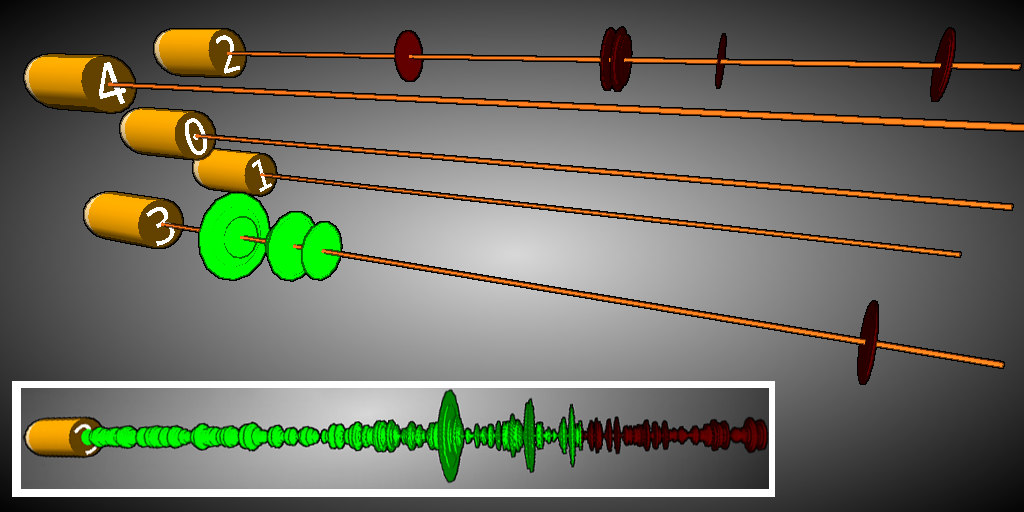
\includegraphics[width=\columnwidth, height=0.4\columnwidth]{figures/recording-3dsound}}
    \caption{Combining the spatial orientation and layout of the recording electrodes with the temporal signal relieves the surgeon of the burden to keep this association in mind. To enhance the perception of the spikes, only the values above a certain threshold are shown in this view so that they are visible pre-attentively. The inset shows the result for one electrode without thresholding.}
    \label{fig:recordingphase:3dsound}
\end{figure}

Creating a disc for every measurement point would clutter the whole view (see inset in Figure~\ref{fig:recordingphase:3dsound}). Therefore we apply the same thresholding technique as described in the previous section, but discard all signals below the threshold completely.

%\subsection{Placement Phase}\label{sec:overview:placement}
%In the placement phase the surgeon needs to consider all acquired information to determine the optimal position of the stimulating electrode. This decision is based on three different factors that are all affected by varying uncertainties:

First, the surgeon's experience and knowledge in selecting and segmenting the intended target region during the planning phase. The segmentation is uncertain as, for example, the brain shifts from its scanned position during the operation. There exist techniques to reduce this uncertainty and we estimate it by measuring the difference between the expected electrode position and the reconstructed position based on the x-ray images. Second, the results of the MER recording and the area along the trajectory. The uncertainty for this step is highly dependent on both the algorithm used to analyze the MER signal and the electrode configuration. The third factor is acquired when the stimulating electrode is inserted and activated. The surgical staff will test different brain functions of the patient. Since it is well-known which areas affect which capabilities while stimulated, the surgeon can further narrow down the location of the optimal target region. In our example we use two brain functions, the ability to recall events from long-term memory and an increase in tremor of the patient's hand. Each of the functions is tested separately along the access path and, based on the surgeon's experience and a patient-neutral heuristic, it is possible to deduce the target region's position relative to the measurement point. The level of uncertainty for this information is relatively constant and in the same range as the extent of the electrodes,$< 1.5 mm$ for our setup. For each decision factor we independently measure the probability, and uncertainty, of the target region's position along the access path.

The contextual view introduced above is shown to maintain the surgeon's mental registration. Since the whole trajectory has been measured in the previous phase, however, all beads and all information previously acquired in the canal tube is presented independently of the electrode position. 

\subsubsection{Target Closeup}\label{sec:overview:placement:targetareaview}
\begin{figure}[t]
  \centering
  \fbox{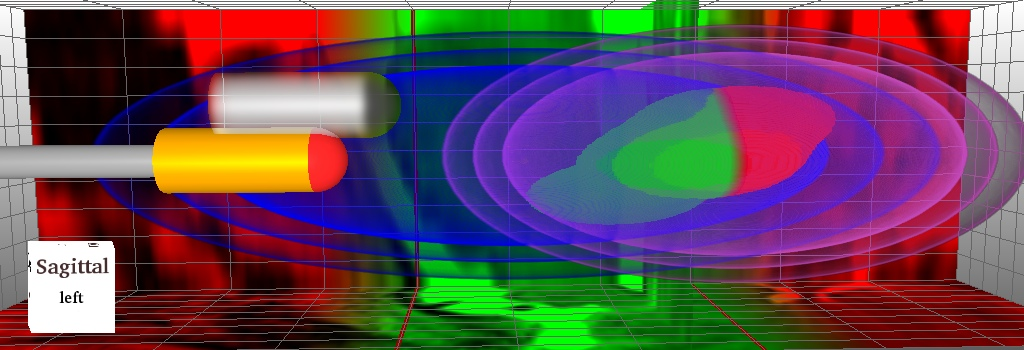
\includegraphics[width=0.98\columnwidth]{figures/electrode_closeup.jpg}}
$%  \fbox{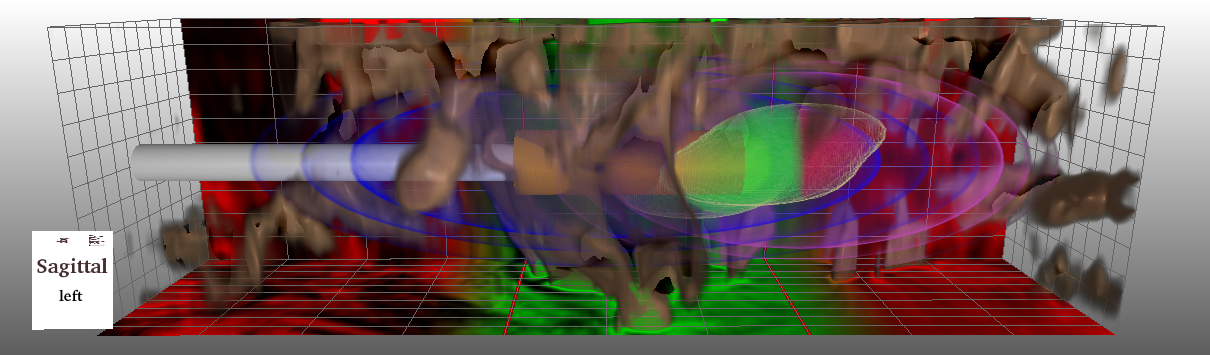
\includegraphics[width=0.98\columnwidth]{figures/target-region_full}}
  \caption{The target closeup visualization shows the potential target regions (speech tests=blue, movement tests=purple). The spatial context provided by the MRI signal is color coded using the red-green MER region mapping. The stimulation electrode changes its color when it is entering the intersection of the potential target area. This view gives qualitative access to all uncertainty data fused with structural data in one glance.}
  \label{fig:targetregion}
\end{figure}

The localization procedure must not only communicate the electrode's position with respect to anatomical structures, but also with regard to the intended target region. An optimal placement of the stimulation electrode should be in the intersection of the potential target regions obtained from the different measurements. We support this in-detail navigation aspect by providing a 3D visualization, which we refer to as the \emph{target closeup}, that shows the electrode embedded in the potential target regions together with the intended target region. To relate these potential target regions to the electrode and embed them into the spatial context, we additionally display the pre-operative MRI scans as a view-dependent projection on the back faces of the target closeup's bounding box. The rendering of the datasets has been made optional as, while it can provide valuable information regarding the intersection between the electrode and structures of interest, it can also occlude the potential target regions. The same orientation overlay, which is also used in the other 3D representations, is used in the electrode closeup to allow a seamless embedding of this view.

We have to deal with three different types of potential target regions, where the type of a region depends on the way it has been acquired. First, the \emph{planned region}, which has been manually defined through segmentation by the surgeon on the basis of the pre-operative MRI scans. Therefore, we can apply volume rendering to show the result of this planning process. The second type is derived from the \emph{MER signal} and has considerable uncertainty. This is projected onto the back planes of the detail view with the color coding that we have also used for visualizing the original MER signal. A safety margin is displayed to account for the occurring uncertainty sources. The third type of potential target region is derived from the \emph{patient tests} performed when placing the stimulating electrode and must, therefore, be interactively changeable. The region is shown as an ellipsoid in 3D assembled by connecting several check points. In the example, shown in Figure~\ref{fig:targetregion}, we depict the ellipsoid generated from multiple speech tests in yellow, while the ellipsoid obtained from the movement tests is depicted in blue. The safety margins are depicted by using transparency, as it allows them to be communicated intuitively while still maintaining a moderate level of occlusion. The width of the safety margins is dependent on experience and the electrode configuration that is used in the intervention.

Similarly to the contextual view, we make it possible for the surgeon to show the approximate location of the electrode as reconstructed from the x-ray scans. This is of particular interest in this view, as it shows the deviation of the actual position from the predicted electrode position, due to brain shift and bending of the needle. The uncertainty of the reconstruction is shown by blurring the rendering of the electrode to fill the size of the uncertain region.

Finally, we emphasize the intersection of the displayed target regions as this intersection is the region where an optimal electrode placement would occur. We compute this intersection interactively and display it volumetrically with a green hue, the same as is used for the green-to-red MER mapping. Thus, the surgeon can verify the overlap and decide in which region to place the electrode. Furthermore, through the extent of the red region, the surgeon gets information about the mismatch between the pre-operative planning and the MER recordings. To further guide the surgeon during the electrode placement, we additionally change the color of the electrode when it penetrates the computed interaction of the potential target regions.

\subsubsection{Placement Guide}\label{sec:overview:placement:guide}
\begin{figure}[t]
  \centering
  \fbox{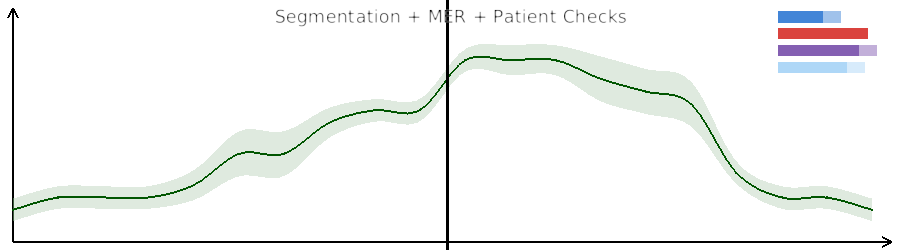
\includegraphics[width=0.96\columnwidth]{figures/segmentation_mer_patientchecks.png}}
%  \fbox{\includegraphics[width=0.465\columnwidth]{figures/individual.png}}
%  \fbox{\includegraphics[width=0.465\columnwidth]{figures/segmentation_mer.png}}\\
%  \fbox{\includegraphics[width=0.465\columnwidth]{figures/segmentation_patientchecks.png}}
%  \fbox{\includegraphics[width=0.465\columnwidth]{figures/mer_patientchecks.png}}
  \caption{The placement guide gives a quantitative overview of measured data for potential target regions. The top figure is a combination of all data values, where as the lower figures present detailed information by showing either all values or pairwise combinations. These combinations enable the surgeon to gain further insight into the measurements in certain situations, for example, when a measurement proves unreliable during the procedure.}
  \label{fig:placementguide}
\end{figure}

In addition to the spatial context, as described in the previous section, we also present the potential target regions quantitatively in a view we call the \emph{placement guide}. This view is centered on the intended target region with the access path depth on the abscissa and the likelihood of the actual target region on the ordinate. By showing the quantitative data in a line plot, the surgeon immediately sees in which areas most of the measurements agree and is guided towards that position. As we have multiple decision values for each depth value, we can combine them in different ways. In our example we chose a weighted sum, but the combination function can be freely changed according to future research. The values for uncertainty are combined in the same way and are rendered as transparent areas surrounding the line. Transparency has been shown to be a good way to convey uncertainty in other contexts~\cite{Djurcilov2002239}. With this representation the size of the transparent area immediately shows how uncertain a specific value is. This lets the surgeon see the whole set of information at one time and decide on an optimal placement position. All combined views use spline-based smoothing on the curves, which can be disabled by the user. This is done so that the surgeon is not distracted by abrupt changes in the data values which would otherwise draw unwanted attention . The current position of the electrode is shown as a bar in each of the views.

The top figure in Figure~\ref{fig:placementguide} shows the combined data of all values and is of central interest for the surgeon. It provides an overview of all measured data and guides the surgeon to the most likely, the highest, position. The curve is assembled while the stimulating electrode is being advanced and the patient checks are performed. Since the combined curve hides possible outliers and gives no feedback on the underlying values, the composition of each sample point can be examined in the top right as a bar plot that shows the probability and uncertainty for each decision factor separately. All bars are justified to the left, with their width directly relating to the measured value. As with the line plot, a transparent box shows the area of uncertain values. One bar is rendered for each source of measurements. So in our case (see Figure~\ref{fig:placementguide}) there is one bar for the segmentation, MER, and one for each of the two patient checks. Including a line alongside the combined data for each of the decision factors would clutter the view and would distract the surgeon too much, which is why we chose to add the bar plot representation. There is,however, an optional view showing those decision factors separately. Furthermore, it is possible to view all pairwise combinations of factors. Showing these auxiliary views, the surgeon can detect outliers and unexpected behavior immediately without distracting him from the main view. Toggling of these auxiliary views can become important in an operation when the surgeon, for example, notices that the patient checks of this particular patient are not as reliable as expected or detects a flaw in the segmentation. Furthermore, it can be useful to inspect the data as if one of the measurements is not considered. This inspection might lead to finding that one of the measurements is not reliable.

%\section{Implementation}\label{sec:implementation}
%In this section we describe selected implementation details of our system.

%\noindent \textbf{Multivolume raycasting.} For the contextual view we need to render registered multimodal datasets and at the same time integrate the electrodes and beads into the rendering. For the rendering we exploit GPU-based volume raycasting as presented by Kr\"uger and Westermann~\cite{kr}. We include the geometric information of objects into this raycasting scheme by modifying the exit points such that the raycasting process ends at those objects~\cite{Scharsach}. The objects are rendered in a separate pass and the results are blended to obtain the final rendering result. To achieve interactive multivolume raycasting we employ a modified version of the region based scene description as presented by Lindholm~et~al.~\cite{Lindholm2009}.

%\noindent \textbf{Skull stripping.} We implemented the skull stripping algorithm as presented by Beyer~et~al.~\cite{Beyer2007}. Although a complete segmentation would provide better results, we want to avoid the necessary user interaction. The basis for this method is opacity peeling~\cite{Rezk-salama2006} which is, in our case, performed on the conditional ray-casting results. Depending on a user-selected parameter, the accumulated values are reset as soon as the early ray-termination criterion is reached. The skull stripping employed in our system uses registered CT and MRI scans to determine the boundary between the brain and the outer layers. Thus, the values accumulated along a ray can be reset when the rays leaves the bone structures and the ray traversal through the brain starts. This method requires no user interaction and provides good and stable results.

\section{Evaluation}\label{sec:evaluation}
As computer-aided surgery systems are combining an increasing number of types of information from different sources, it is important that the interfaces reduce the cognitive load required to use the system~\cite{Visarius1997,Martelli2003}. To evaluate the practicability of the proposed system we have conducted a qualitative user-study with five neurosurgeons, all of whom have extensive experience in the field and perform DBS interventions on a regular basis. The study has been designed with respect to the guidelines for evaluating computer-aided surgery systems, which have been proposed by Martelli et al.~\cite{Martelli2003}. The neurosurgeons were shown a showcase demonstration of the system going through all three phases (planning, recording, and placement). A demonstration was chosen, as a pre-study showed that the complexity of usage, in the current form, would result in a biased evaluation. The data for this demonstration was recorded and reconstructed from a real intervention. After the demonstration the neurosurgeons answered a questionnaire consisting of eight statements and questions, as well as a text field for arbitrary comments. Each of these statements and questions had a positive and a negative reply with no opportunity to abstain. The following table shows all statements and questions together with the number of positive answers:

\noindent \begin{tabular}{p{0.875\columnwidth} c}
\hline
The user is not disturbed by images, colors, or animation while interacting with the system	& 4\\
The result of any action done by the user is clearly and immediately visualized				& 4\\
The tools provided by the system are easy to use												& 3\\
System data is understandable and clearly visualized											& 4\\
The actions' succession proposed by the system is logical from the user's point of view		& 5\\
The system's features are compatible with all the user's expectations							& 4\\
Would you like to use this system during an intervention in addition to the old system?		& 5\\
Is the fusion of MER signals with image data useful for increasing the accuracy?				& 3\\
\hline
\end{tabular}

\noindent \textbf{Discussion.} Overall, the feedback from the neurosurgeons was very positive. The least satisfied expert agreed with only five statements whereas the most satisfied expert agreed to all. On average the experts agreed to $6.5$ statements if we assume an equal weighting of the statements. The relatively bad score of only three positive answers to the last question seems to be the strongest drawback to the method, but considering that all of the experts would use our system in the operation room makes it a good result. One expert emphasized especially the ''correlations between target region and the neurophysiological data'' as an important aspect of the system. Only two neurosurgeons did not see the benefits of incorporating the fused views, while they still liked the overlapping view of the different probable target regions. The third question confirmed the expected usability result from the pre-study.

\section{Conclusions and Future Work}\label{sec:conclusions}
In this paper we have presented a visualization system that has been designed to support neurosurgeons during DBS interventions by fusing measurement data, along with their uncertainties, with structural modalities to facilitate mental registration. This multimodal information is presented to the surgeon during the intervention both in the context of the rendered imaging data, as well as a separate view showing the combination of these measurements. As the MER and patient checks are performed during DBS interventions to improve the localization of the stimulation electrode, we feed back the results of these checks into our system. When displaying and intersecting the potential target regions we take into account the different degrees of uncertainty that result from their acquisition process. This uncertainty-aware information fusion in image space, as well as in a profile plot, enables the surgeon to better assess the electrode placement and detect the optimal electrode placement. To estimate the clinical impact of the presented system we performed a qualitative evaluation with five neurosurgeons who regularly perform DBS interventions. The results indicate that the presented visualization approaches are of great interest and have the potential to improve DBS interventions.

In the future we would like to further improve the presented system based on the feedback we have received from the surgeons during our evaluation. We would especially like to reduce the learning curve currently necessary. Furthermore, it would be beneficial to evaluate its effectiveness in the operation theater. However, a full evaluation requires a lot of effort as it would require the system to be certified for usage in the operation theater. While the current system considers most modalities, the integration of DTI could also be considered in the future. Another source of information we would like to include is the region of the brain that is affected by the stimulation signal, the \emph{volume of tissue activated}. This would simulate the region in the brain that would be influenced by the current electrode position and could thereby function as a prediction as well as a verification tool. While we have currently focused on the recording and placement phases of the DBS intervention, we would also like to extend the system for long term horizontal studies of electrode placements. A major part of this horizontal study would be the ability to compare the measured accuracy with the outcome of the intervention. As no extensive statistics about the long term effects of varying placement positions and the applied electric fields exist, this could be valuable information for further improving DBS interventions in the future.

\section{Medical Benefits}\label{sec:benefits}
\fix{Workflow instead of System Setup?}
\fix{Focus, Evaluation, no FDA approval}

\section{Conclusions}\label{sec:conclusions}
\fix{Post-Processing for evaluation of technique}

\section*{Acknowledgements}This work was partly supported by grants from the Excellence Center at Link�ping and Lund in Information Technology (ELLIIT) and the Swedish e-Science Research Centre (SeRC), as well as VR grant 2011-4113. The presented concepts have been realized using the Voreen framework (www.voreen.org).

\bibliographystyle{eg-alpha-doi}

\bibliography{literature}


\end{document}